% Simple geometric coding-theory logo
% Standalone TikZ source for presentation/tikzs/logo-coding-geometric.pdf
\documentclass[tikz, border=0pt]{standalone}

\usepackage{xcolor}
\usetikzlibrary{arrows.meta, calc}

\definecolor{inkC}{HTML}{10202A}
\definecolor{paperC}{HTML}{F8FBFC}
\definecolor{gridC}{HTML}{DCEAEC}
\definecolor{codeC}{HTML}{008C8C}
\definecolor{codeDarkC}{HTML}{006A70}
\definecolor{errC}{HTML}{D33F49}

\begin{document}
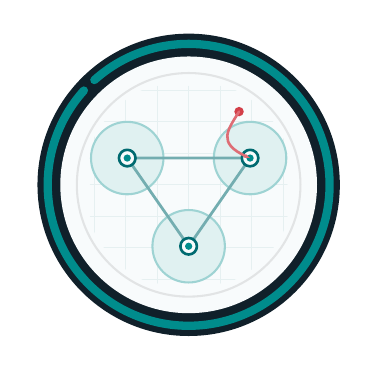
\begin{tikzpicture}[
  x=1cm,
  y=1cm,
  line cap=round,
  line join=round
]

\coordinate (A) at (-0.78,0.34);
\coordinate (B) at (0.78,0.34);
\coordinate (C) at (0,-0.78);
\coordinate (R) at (0.64,0.93);

% Badge
\fill[inkC] (0,0) circle (1.92);
\fill[paperC] (0,0) circle (1.63);
\draw[codeC, line width=3.0pt] (138:1.79) arc[start angle=138, end angle=492, radius=1.79];
\draw[inkC!12, line width=0.75pt] (0,0) circle (1.42);

% Sparse ambient grid
\begin{scope}
  \clip (0,0) circle (1.34);
  \foreach \x in {-1.2,-0.8,...,1.2}{
    \draw[gridC!72, line width=0.32pt] (\x,-1.25) -- (\x,1.25);
  }
  \foreach \y in {-1.2,-0.8,...,1.2}{
    \draw[gridC!72, line width=0.32pt] (-1.25,\y) -- (1.25,\y);
  }
\end{scope}

\begin{scope}[shift={(A)}]
%	\fill[paperC] (0,0) circle (0.86);
%	\fill[matrixC!8] (0,0) circle (0.76);
%	\draw[matrixC!25, line width=4.2pt] (0,0) circle (0.78);
%	\draw[matrixC, line width=1.35pt] (0,0) circle (0.86);
	
	\pgfmathsetmacro{\mxs}{0.135}
	\pgfmathsetmacro{\mys}{0.145}
	\pgfmathsetmacro{\mxo}{-3.0*\mxs}
	\pgfmathsetmacro{\myo}{1.5*\mys+0.10}
	
%	\foreach \col in {3,6,...,15}{
%		\foreach \row in {-2,-1,...,11}{
%			\draw[codeC!38, line width=0.34pt]
%			({\mxo+\col*\mxs-0.042},{\myo-\row*\mys-0.042}) rectangle
%			({\mxo+\col*\mxs+0.042},{\myo-\row*\mys+0.042});
%		}
%	}
%	\foreach \col/\row in {
%		3/-2,
%		3/0
%	}{
%		\fill[codeDarkC] ({\mxo+\col*\mxs},{\myo-\row*\mys}) circle (0.030);
%	}
%	\foreach \col/\row in {0/3,1/2,5/0,6/1}{
%		\fill[paperC] ({\mxo+\col*\mxs},{\myo-\row*\mys}) circle (0.027);
%		\draw[codeDarkC!70, line width=0.45pt]
%		({\mxo+\col*\mxs},{\myo-\row*\mys}) circle (0.027);
%	}
\end{scope}

% Hamming balls around codewords
\foreach \P in {A,B,C}{
  \fill[codeC!12] (\P) circle (0.46);
  \draw[codeC!38, line width=0.75pt] (\P) circle (0.46);
}

%% Voronoi-like decoding boundaries
%\draw[inkC!16, line width=1.05pt] (0,1.10) -- (0,-1.10);
%\draw[inkC!16, line width=1.05pt] (-1.08,-0.24) -- (0.88,1.02);
%\draw[inkC!16, line width=1.05pt] (1.08,-0.24) -- (-0.88,1.02);

% Code geometry
\draw[codeDarkC!55, line width=1.0pt] (A) -- (B) -- (C) -- cycle;
\foreach \P in {A,B,C}{
  \fill[paperC] (\P) circle (0.105);
  \draw[codeDarkC, line width=0.95pt] (\P) circle (0.105);
  \fill[codeC] (\P) circle (0.046);
}

% Central parity/syndrome mark
%\fill[inkC] (0,0) circle (0.18);
%\foreach \ang in {90,210,330}{
%  \fill[paperC] (\ang:0.095) circle (0.030);
%}

% Received word corrected to nearest codeword
\fill[errC] (R) circle (0.060);
\draw[errC!76, line width=0.95pt, -{Stealth[length=2.15pt]}]
  (R) .. controls (0.50,0.70) and (0.35,0.53) .. (B);

%% Small coordinate/codeword row hint
%\draw[codeC!45, line width=0.75pt] (-0.58,-1.18) -- (0.58,-1.18);
%\foreach \x/\filled in {-0.48/1,-0.32/0,-0.16/1,0/1,0.16/0,0.32/0,0.48/1}{
%  \ifnum\filled=1
%    \fill[codeC] (\x,-1.18) circle (0.040);
%  \else
%    \fill[paperC] (\x,-1.18) circle (0.040);
%    \draw[codeC, line width=0.65pt] (\x,-1.18) circle (0.040);
%  \fi
%}

\end{tikzpicture}
\end{document}
